\section{Overview}
This analysis searches for exotic decays of the Higgs boson (\PH) using data collected by the CMS experiment (Chapter~\ref{ch:cms}) from the \pp collisions produced at the CERN LHC (Chapter~\ref{ch:lhc}) at a center-of-mass energy of 13\TeV during the Run 2 period (2016--2018).
Two different decay mechanisms are considered: \htozx and \htoxx.
Here, \PX represents a BSM particle that decays into a pair of OSSF leptons, though only electrons and muons are considered.
Because the \PZ is the SM \PZ boson, this decay process yields the same four-lepton (\fourl) final states that were found in the Higgs boson mass measurement analysis (Chapter~\ref{ch:higgs_mass}):
\foure, \fourmu, \twoetwomu, and \twomutwoe.
The \fourl final state was chosen due to its clean signature and large signal-to-background ratio.

Within the theoretical framework of the ``Hidden Abelian Higgs Model'' (HAHM) (TODO:refs7--11 from EJPC), the BSM particle \PX is speculated to interact with SM particles via the ``dark'' sector.
In this model, \PX is the dark photon $\left( \PZD \right)$ and mediates a dark $U(1)_\text{D}$ gauge symmetry that is spontaneously broken by a theoretical dark Higgs mechanism.

The search for \PZD begins with a SM decay of \htozznostar.
Then, via the dark sector, one of the \PZ bosons \emph{mixes} with \PZD, as determined by the kinetic-mixing parameter $\varepsilon$.
Next, the \PZD and the \PZ bosons both decay into OSSF lepton pairs to yield one of the four different \fourl final states.
This decay process is shown in Fig.~\ref{fig:feyn_diag_hzzd4l_hzdzd4l} (A).
The other mode of \PZD production occurs when \PH mixes with a dark Higgs boson ($s$), as governed by the Higgs-mixing parameter $\kappa$.  % TODO:get fancier kappa
In this case, the $s$ decays into two identical \PZD particles which decay promptly to give one of the \fourl final states.
This decay process is shown in Fig.~\ref{fig:feyn_diag_hzzd4l_hzdzd4l} (B).
%=== Suzanne's Feynman diagram code. ===%
% \begin{figure}[ht]
%     \centering
%     \begin{tikzpicture}
%     \begin{feynman}[large]
%         \vertex (h) {$h$}; % h at beginning 
%         \vertex [right=1cm of h] (ZZ); % h -> ZZ vertex
%         \node [circle, fill=black, inner sep=2pt, above right = 1cm and 1.25cm of ZZ] (Z1); % black dot node at epsilon (control size with ) 
%         \node [above left = 7pt and 7pt of Z1] (e) {$\epsilon$}; % node with epsilon text
%         \vertex [below right = 1cm and 2.5cm of ZZ] (Z2); % h -> ZZ bottom Z
%         \vertex [above right = 0.5cm and 1.25cm of Z2] (Z2l1) {$l$}; % bottom Z -> ll (top l)
%         \vertex [below right = 0.5cm and 1.25cm of Z2] (Z2l2) {$l$}; % bottom Z -> ll (bottom l)
%         \vertex [above right = 1cm and 1.25cm of Z1] (ZD); % ZD
%         \vertex [above right = 0.5cm and 1.25cm of ZD] (ZDl1) {$l$}; % ZD -> ll (top l)
%         \vertex [below right = 0.5cm and 1.25cm of ZD] (ZDl2) {$l$}; % ZD -> ll (bottom l)
%         \diagram* {
%             (h) -- [scalar] (ZZ),
%             (ZZ) -- [boson, edge label=$Z$] (Z1),
%             (ZZ) -- [boson, edge label=$Z$] (Z2),
%             (Z1) -- [boson, edge label=$Z_D$] (ZD),
%             (ZDl2) -- [fermion] (ZD) -- [fermion] (ZDl1);
%             (Z2l2) -- [fermion] (Z2) -- [fermion] (Z2l1);
%         };
%     \end{feynman}
%     \end{tikzpicture}
% \end{figure}
% \newpage
% \begin{figure}[ht]
%     \centering
%     \begin{tikzpicture}
%     \begin{feynman}[large]
%         \vertex (h) {$h$}; % h at beginning 
%         \node [circle, fill=black, inner sep=2pt, right=1.5cm of h] (kappa); % black dot at kappa node
%         \node [above left = 7pt and 7pt of kappa] {$\kappa$}; % node with kappa text
%         \vertex [right=1.5cm of kappa] (s); % s -> ZDZD vertex
%         \vertex [above right = 2cm and 1cm of s] (Z1); % top ZD
%         \vertex [below right = 2cm and 1cm of s] (Z2); % bottom ZD
%         \vertex [above right = 0.5cm and 1.25cm of Z2] (Z2l1) {$l$}; % top l of top Z
%         \vertex [below right = 0.5cm and 1.25cm of Z2] (Z2l2) {$l$}; % bottom l of top Z
%         \vertex [above right = 0.5cm and 1.25cm of Z1] (Z1l1) {$l$}; % top l of bottom Z
%         \vertex [below right = 0.5cm and 1.25cm of Z1] (Z1l2) {$l$}; % bottom l of bottom Z
%         \diagram* {
%             (h) -- [scalar] (kappa),
%             (kappa) -- [scalar, edge label=$s$, below] (s),
%             (s) -- [boson, edge label=$Z_D$] (Z1),
%             (s) -- [boson, edge label=$Z_D$] (Z2),
%             (Z1l2) -- [fermion] (Z1) -- [fermion] (Z1l1);
%             (Z2l2) -- [fermion] (Z2) -- [fermion] (Z2l1);
%         };
%     \end{feynman}
%     \end{tikzpicture}
% \end{figure}
%%%%%%%%%%%%%%%%%%%%
% H->Z(Zd)Zd->4L Feynman Diagrams.
%%%%%%%%%%%%%%%%%%%%
\begin{multiFigure}
    % \begin{figure}[pbth]
        \centering
        % 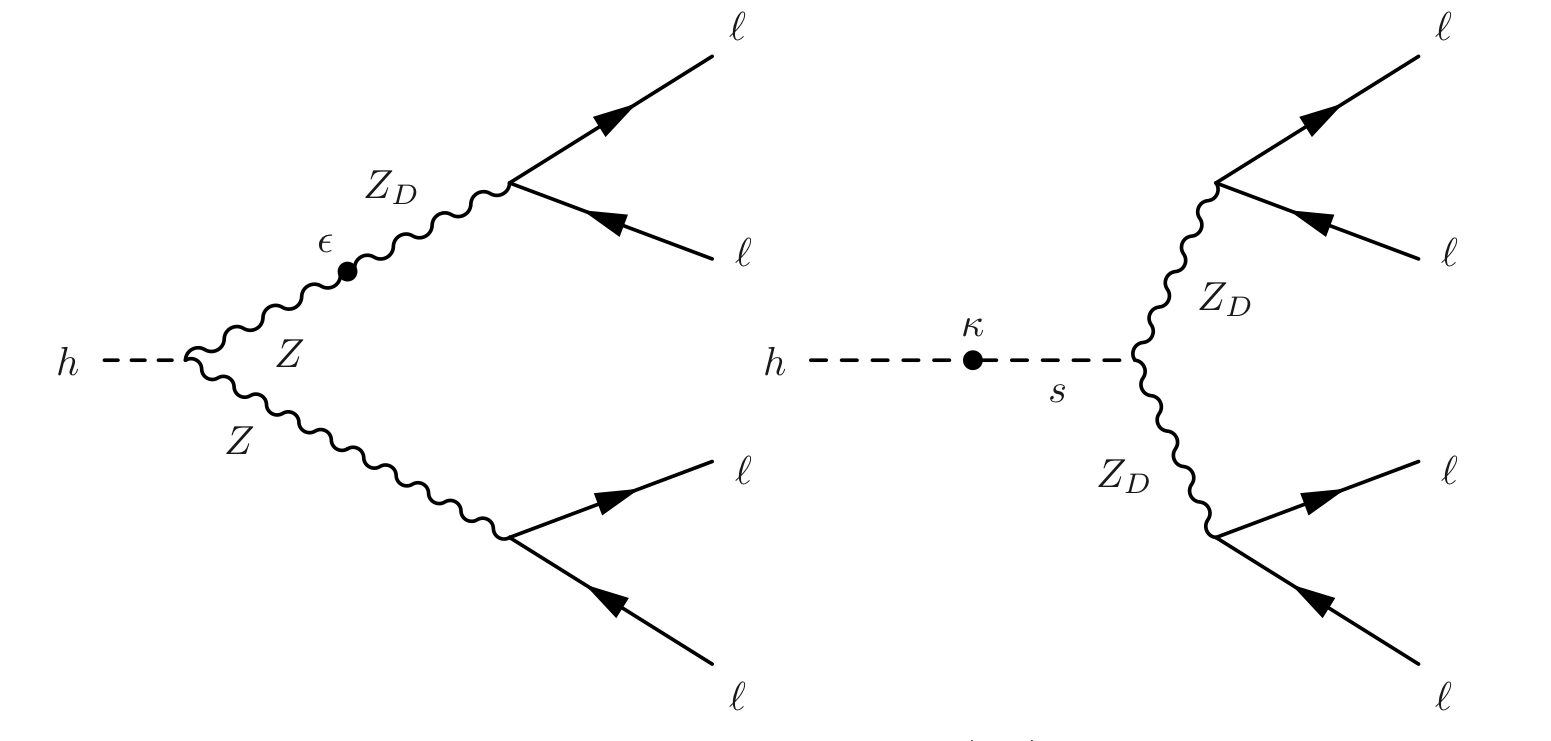
\includegraphics[height=8cm]{figures/dilep_res/feynman_diagram_hzzd4l_hzdzd4l.jpeg}
        \addFigure{0.48}{figures/dilep_res/feynman_diagram_hzzd4l.pdf}
        \addFigure{0.48}{figures/dilep_res/feynman_diagram_hzdzd4l.pdf}
        \captionof{figure}
            [Exotic decays of the Higgs boson to the \fourl final state.]
            {Exotic decays of the Higgs boson ($h$) to the \fourl final state within the context of the HAHM.
            A) Higgs boson decays into two SM \PZ bosons, one of which kinetically mixes with the dark photon $\left(\PZD\right)$.
            B) Higgs boson mixes with a dark Higgs boson ($s$) via the Higgs-mixing mechanism, governed by the Higgs-mixing parameter $\kappa$.
            The dark Higgs then decays into two identical dark photons, each of which decays into two OSSF leptons.}
        \label{fig:feyn_diag_hzzd4l_hzdzd4l}
\end{multiFigure}

This analysis assumes a narrow-width approximation for \PZD decays so that the dark photon is confined to its on-mass shell.
Thus, for any given dark photon mass hypothesis, \PZD is assumed to always have that singular mass value.
This limitation on the mass of \PZD $\left(\mZD\right)$ in conjunction with the narrow-width nature of the Higgs boson mass resonance $\left( \mH \approx 125\GeV \right)$ kinematically constrains the search region of the analysis.
Specifically, the \htozzd $\left(\htozdzd\right)$ process has the upper limit
$\mZD < \mH - \mZ \approx 35\GeV    \left(\mZD < \mH / 2 \approx 62.5\GeV\right)$.
Finally, to avoid the ubiquitous but unwanted reconstruction of intermediate mass resonances that often decay into dilepton final states,
like the $\jpsi$ $\Pc\Pac$ bound state meson $\left( \mass{\jpsi} \approx 3.1\GeV \right)$~\cite{particle_data_group_review_2020}
% More precise J/psi mass: 3.096\,900 \pm 0.000\,006\GeV
and the $\varUpsilon$ $\bbbar$ bound state meson $\left( \mass{\varUpsilon} \approx 10.0\GeV \right)$~\cite{particle_data_group_review_2020},
the mass range chosen for this analysis is $4.0 < \mZD < 35.0\GeV \left(62.5\GeV\right)$ while excluding the mass window $8.0 < \mass{\varUpsilon} < 11.5\GeV$.

The search for \PZD uses many of the same procedures found in the Higgs boson mass measurement analysis detailed in Chapter~\ref{ch:higgs_mass}.
However, the search for \PZD uses ``ReReco'' reconstruction instead of Ultra Legacy, since the Ultra Legacy reconstruction was not available at the time.
The trigger paths used to select relevant \pp collision data are given in Sec.~\ref{sec:trig_dilep}.
The names of the data sets used along with their corresponding \lumiint are detailed in Sec.~\ref{sec:datasets_dilep}.
Finally, the details of the data sets that contain the relevant simulated events are listed in Sec.~\ref{sec:sim_samples_dilep}.

The event selection for the search for \PZD (Sec.~\ref{sec:evt_sel_dilep}) is very similar to the event selection outlined in (Sec.~\ref{sec:evt_sel}), with just a few differences to optimize for the selection of low-mass dilepton candidates.
In particular, since low-mass dilepton candidates are desired must have an invariant mass that falls outside the mass window corresponding to the $\varUpsilon$ \bbbar bound states $\left( 8.0 < \mass{\varUpsilon} < 11.5\GeV \right)$. 
In the \zdzd search, \mZone and \mZtwo must be between 4\GeV and 62.5\GeV.

As much as particle physicists hoped to observe the so-called ``golden channel'' $\left( \hzzfourl \right)$
% , in which the SM Higgs boson decays into the \fourl final state,
this analysis is---\emph{ironically}---contaminated by the golden channel!
Thus, the irreducible background processes for this analysis include \htofourl decays, rare backgrounds such as $\ttbar + \PZ$ and triboson production, along with the same processes described in Sec.~\ref{sec:bkg_irred}.
Furthermore, the reducible background (RB) processes are exactly the same as those mentioned in Sec.~\ref{sec:redbkg}.
The OS method (Sec.~\ref{sec:os_method}) is again used to estimate the contribution from RB processes.
A summary of the analysis of the background processes and misidentification rates of leptons is given in Sec.~\ref{sec:bkg_estim_dilep}.

% syst_uncert
% results
